\documentclass[10pt]{beamer}
\usetheme{default}
\setbeamertemplate{navigation symbols}{}
\setbeamertemplate{footline}
{
  \leavevmode%
  \hbox{%
  \begin{beamercolorbox}[wd=.40\paperwidth,ht=2.5ex,dp=1ex,center]{author in head/foot}%
    \usebeamerfont{author in head/foot}\insertshortauthor
  \end{beamercolorbox}%
  \begin{beamercolorbox}[wd=.50\paperwidth,ht=2.5ex,dp=1ex,center]{title in head/foot}%
    \usebeamerfont{title in head/foot}\insertshorttitle
  \end{beamercolorbox}%
  \begin{beamercolorbox}[wd=.10\paperwidth,ht=2.5ex,dp=1ex,center]{date in head/foot}%
    \insertframenumber{} /\inserttotalframenumber\hspace*{1ex}
  \end{beamercolorbox}}%
  \vskip0pt%
}
\makeatletter

\usepackage[T1]{fontenc}
%\usepackage[utf8]{inputenc}
%\usepacage[italian]{babel}
\usepackage{amsmath} % allows to use \text in arrays
\usepackage{afterpage} % Execute command after the next page break
\usepackage{syntonly}
%\syntaxonly
\usepackage{changepage}
\usepackage{comment}

%Tables and figures
\usepackage{tabularx} % introduces column type X
\usepackage{array}
\usepackage{rotating} % per ruotare tabelle grandi
\usepackage{longtable}
\usepackage{siunitx} % gestisce in modo molto potente e flessibile anche la resa tipografica dei numeri nelle tabelle, definendo un nuovo tipo di colonna S specifica per dati numerici
\sisetup{output-decimal-marker={.},input-symbols = ()} % "(" and ")" are ordinary inputs
\setbeamertemplate{caption}[numbered]
\setbeamerfont{framesubtitle}{size=\large}
\usepackage[compatibility=false]{caption}
\captionsetup{tableposition=top,figureposition=bottom,font=scriptsize}
\usepackage{subcaption}
\captionsetup[sub]{font=scriptsize,labelfont={bf,sf}}
\usepackage{booktabs} % per tabelle
\usepackage{graphicx} % per figure
\usepackage{pgfplots}
\pgfplotsset{width=\textwidth,compat=1.11}
\usepackage{adjustbox}
\usepackage{tikz}
\usetikzlibrary{calc}
\graphicspath{{../paper/}{../figures/}{../}}
\usepackage{threeparttable}

%New command for captions below the table (in addition to those above)
\newcommand\fnote[1]{\captionsetup{format=plain,font=footnotesize,justification=justified}\caption*{#1}}
\newcommand{\B}[1]{{\color{blue} #1}}
\newcommand{\G}[1]{{\color{gray} #1}}
\hypersetup{colorlinks=true, breaklinks=false, linkcolor=gray, menucolor=gray, urlcolor=blue, citecolor=gray}

%Symbols
\usepackage{pifont}% http://ctan.org/pkg/pifont
\newcommand{\cmark}{\ding{51}}%
\newcommand{\xmark}{\ding{55}}%

%% Referencing
\usepackage{hyperref}
%\usepackage{breqn}
%\usepackage{amsmath}

%% Citations
%\usepackage[authoryear]{natbib}
%\usepackage{hyperref}
%\citestyle{apacite}
%\def\bibfont{\small}

%Biblio
\usepackage[style=authoryear-comp,backend=bibtex,uniquename=init,firstinits,maxcitenames=2,natbib=true,url=false,doi=false,eprint=false]{biblatex}
\bibliography{bibliography}

\title[Institutions and innovation]{Institutions and Innovation: \\ Evidence from the Italian Unification}

\author[Domini \& Machielsen]{Giacomo Domini\inst{} 
    \and Bas Machielsen\inst{}}

\institute{
    \inst{} Utrecht University School of Economics}
    
\date[Sep 2024]{9th ASE Annual Meeting, 14 September 2024}

\begin{document}

\begin{frame}
  \titlepage
\end{frame}

\begin{frame}
    \frametitle{Introduction}
    
    Innovation seen at the basis of economic growth \citep{schumpeter1942, solow1957} \\  \bigskip
    
    Innovation is a \textit{proximate} cause of economic growth; it is itself determined by \textit{fundamental} causes, most importantly institutions \citep{acemoglu2005, north1973, north1990} \\    \bigskip
    
    \pause
    
    19th-century Europe: many episodes of institutional change, at a time in which the First Industrial Revolution spread and the Second  started \\    \bigskip

    We focus on an episode from Italy's unification process (1850-60s), namely the annexation of Lombardy to Piedmont from Austria:
    
    \begin{itemize}
        \item Significant shift towards liberal institutions
        \item Quasi-random assignment, based on military circumstances
    \end{itemize}

    \bigskip
    
    Not only of historical relevance, at an age characterised by serious challenges to the liberal-democratic global order 
    
\end{frame}

\begin{frame}
    \frametitle{Relevant literature}
    
    Institutions and growth: old question \citep{delong1993}, boost after \cite{acemoglu2001, acemoglu2002} \citep{rodrik2004, aghion2007} \\  \bigskip

    Institutions and innovation: %(Donges et al., 2022; Acemoglu \& Johnson, 2023)
    \begin{itemize}
%        \item National innovation systems \citep{freeman1987, lundvall1992, nelson1993}
        \item Democracy and innovation \citep[the "Popper" hypothesis][]{gao2017}: \cite{aghion2007, acemoglu2019, gao2017, wang2021}
        \item Patent systems and innovation: \cite{moser2005, lerner2009}
        \item Social institutions and innovation: \cite{greif2012}
        \item Access to useful knowledge and innovation: \citep{buonanno2024}
        \item ``High-level'' institutions: \cite{donges2022}
        \begin{itemize}
            \item Closest to us i.t.o. type of institutions and identification strategy 
        \end{itemize}
    \end{itemize}
    
    \bigskip

    \pause

    Innovation in Italy in the very long run \citep{barbielliniamidei2013, nuvolari2015b}:
    \begin{itemize}
        \item micro evidence at province \citep{nuvolari2018}, municipality \citep{buonanno2024}, firm \citep{domini2023}, and entrepreneur level \citep{toninelli2014, nuvolari2018, domini2019}
        \item few analyses go before unification \citep{nuvolari2019, nuvolari2020}
        %\item long period by international standards \citep{bergeaud24, petralia16} 
    \end{itemize}
    
\end{frame}

\begin{frame}
    \frametitle{Historical context}
    
    \begin{figure}
        \centering
        \includegraphics[width=0.5\linewidth]{maps/stati_preunitari.png}
        \caption{Italy in 1848}
        \label{fig:map_italy_1848}
    \end{figure}
    
\end{frame}

\iffalse
\begin{frame}
    \frametitle{Historical context}
    
    \begin{figure}
        \centering
        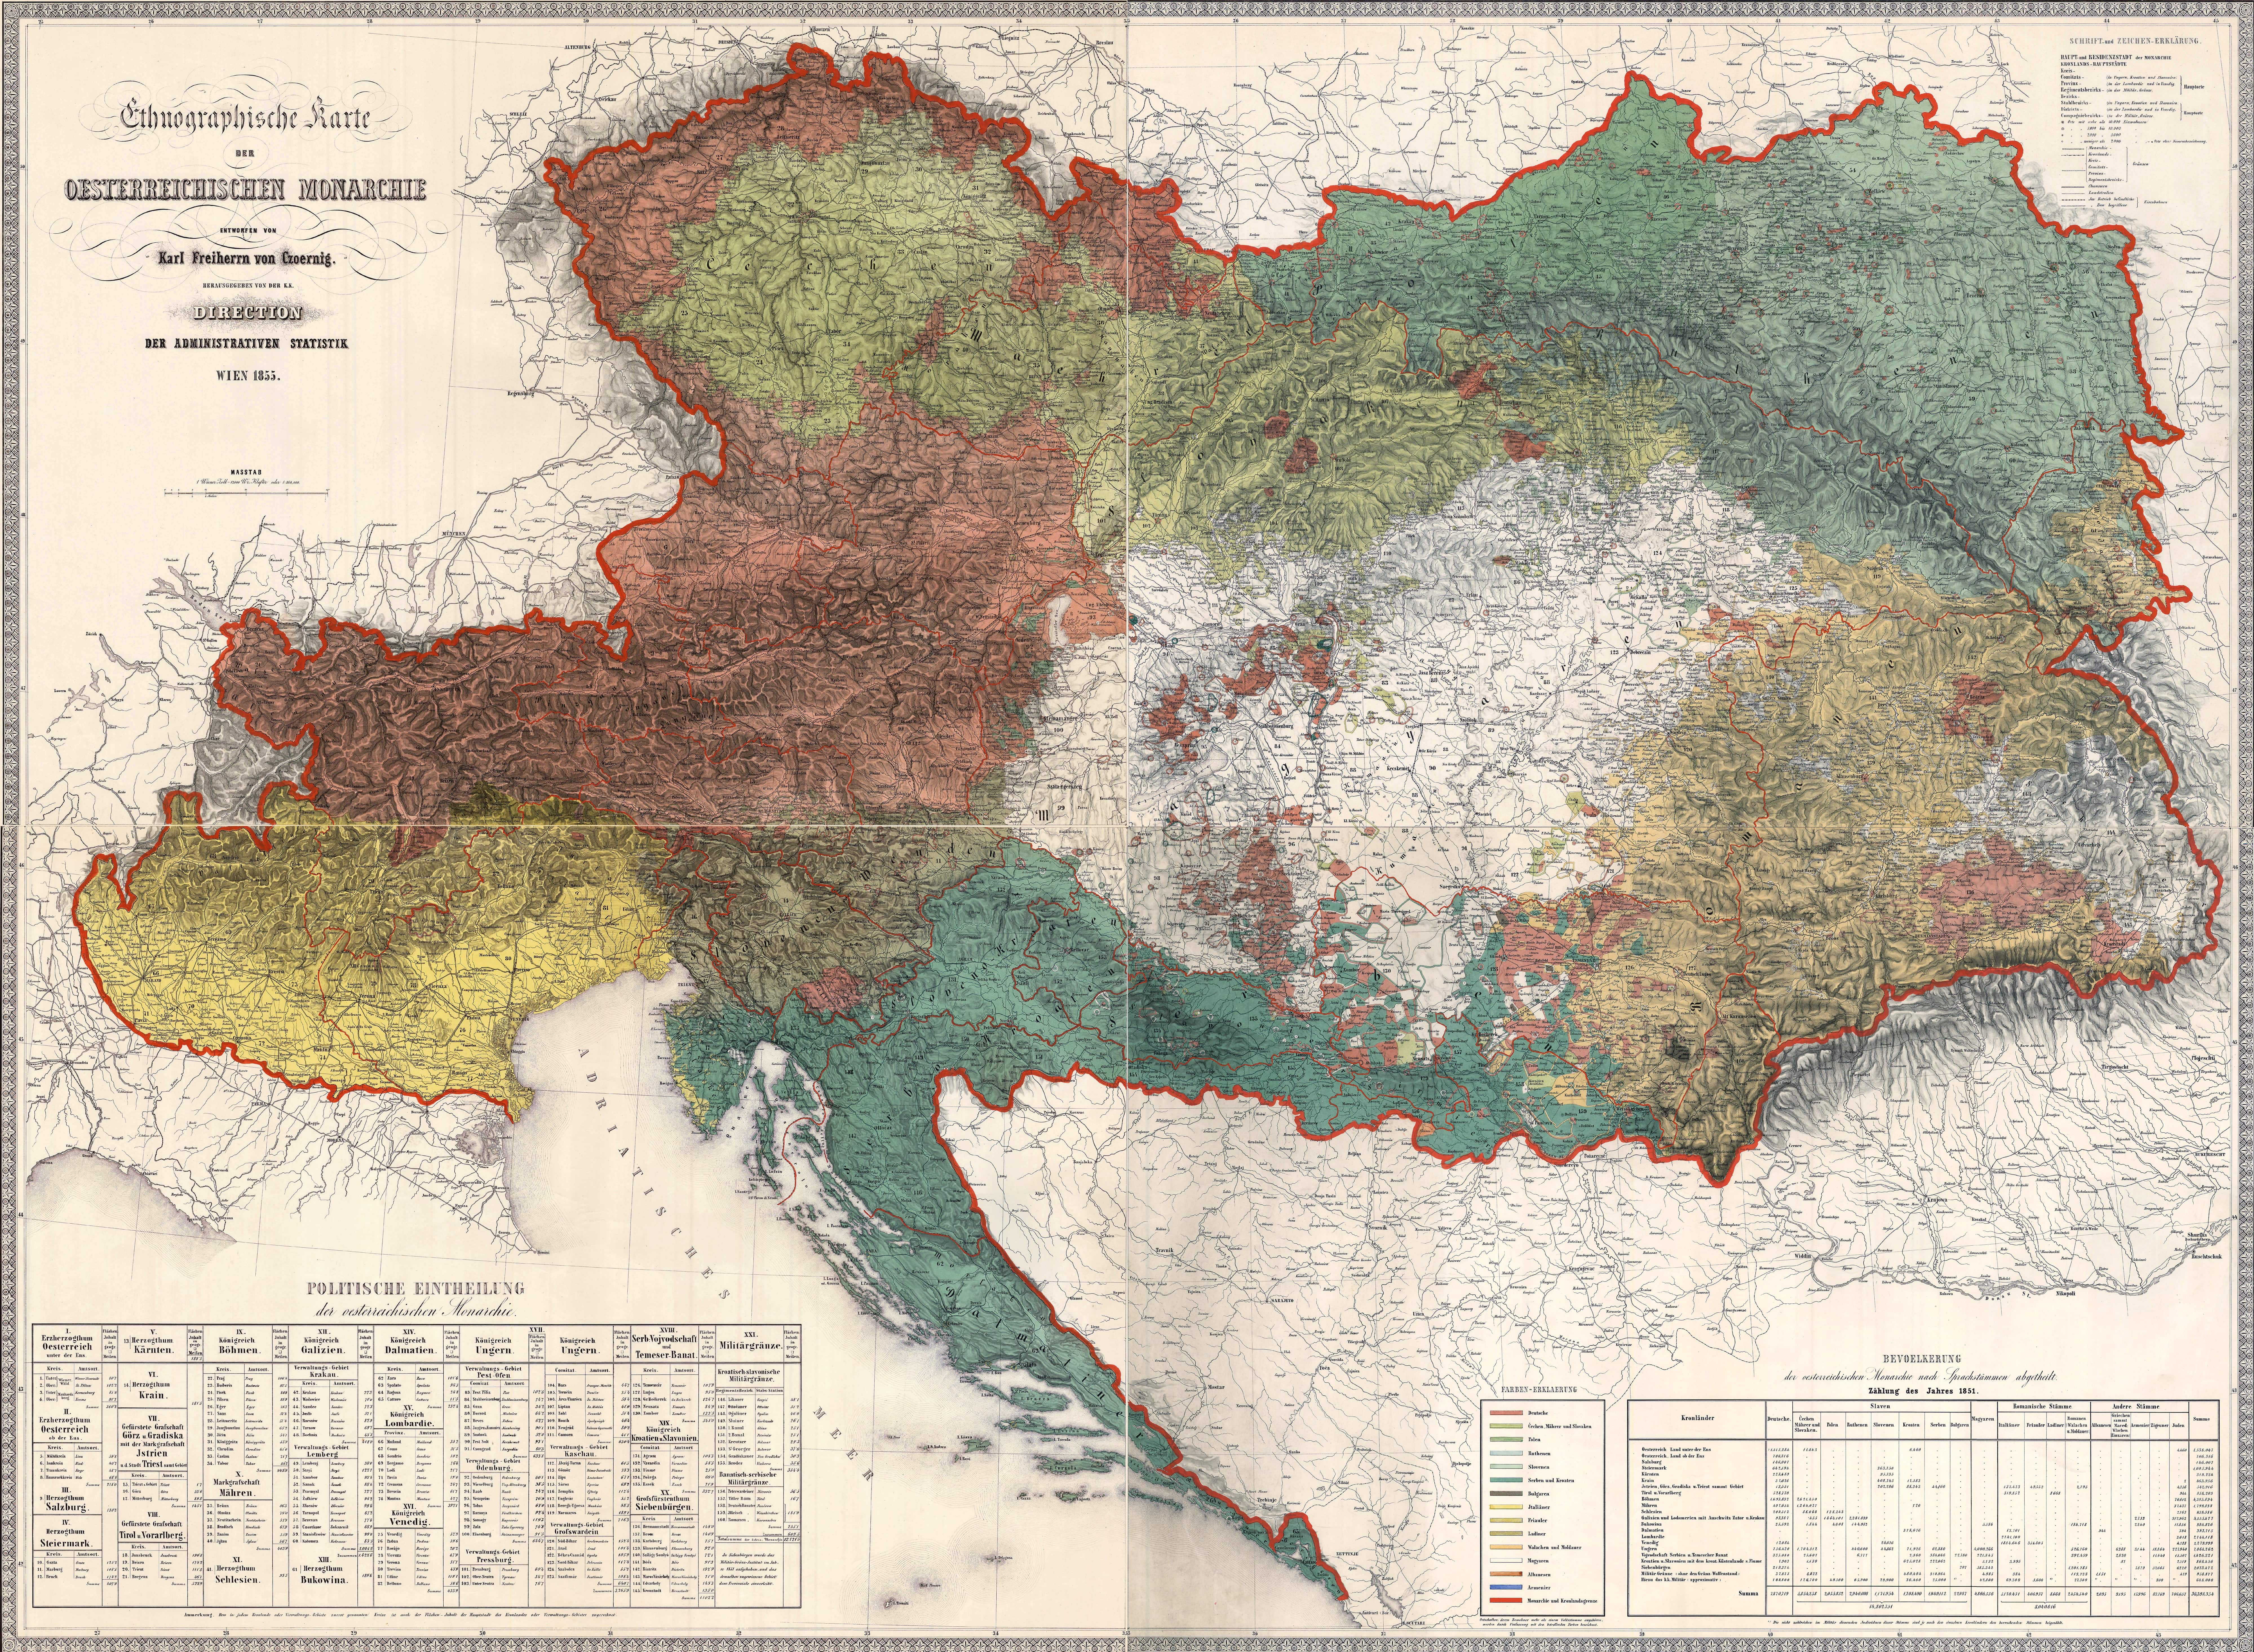
\includegraphics[width=0.75\linewidth]{maps/austrian_empire_1855.jpg}
        \caption{The Austrian empire in 1855}
        \label{fig:map_austria_1855}
    \end{figure}
    
\end{frame}
\fi

\begin{frame}
    \frametitle{Historical context}
    
    \begin{figure}
        \centering
        \includegraphics[width=0.75\linewidth]{maps/lombardy_venice}
        \caption{The Lombardo-Venetian kingdom}
        \label{fig:map_lombardy_venice}
    \end{figure}
    
\end{frame}

\begin{frame}
    \frametitle{Historical context}
    
    \begin{itemize}
%        \item Italy last united under Justinian (mid-6th c.)
        \item Fragmented since Roman Empire's fall, but flourishing until 15th c.
        \item Long political and economic decline in early modern period $\rightarrow$ Ruled by France, Spain, Austria
        \item In the wake of the French Revolution, growing sentiment in favour of national independence and unification (\textit{Risorgimento})
%        \pause
        \item 1848-1849: uprisings and first war of independence (lost)
        \item \textbf{1859: second war of independence $\rightarrow$ Lombardy joins Piedmont}
        \item 1860: Garibaldi conquers the South
        \item 1860: plebiscites across the peninsula to join Piedmont
        \item 1861: Vittorio Emanuele II proclaimed King of Italy
        \item 1866: third war of independence: Veneto joins
        \item 1870: Rome is captured and becomes capital
        \item Post-WWI: Trento and Trieste join
    \end{itemize}
    
\end{frame}

\begin{frame}
    \frametitle{Historical context: the second war of independence}
    
    Piedmont (formally the Kingdom of Sardinia) led the unification:
    \begin{itemize}
        \item Stable monarchy of the House of Savoy
        \item The only Italian state not to repeal the constitution in 1848-9
        \item Liberalism, free trade, compulsory universal schooling (since 1859)
    \end{itemize}

    \pause
    
    \bigskip

    Plombières agreement (1858) and Franco-Piedmontese military alliance (1859): France would help freeing the Lombardo-Venetian kingdom and get Savoy and Nice as reward

    \bigskip
    War fought over 2.5 months (25/4-12/7/1859)
    \begin{itemize}
        \item Austria first enters Piedmont, then retreats as French and Piedmontese advance
        \item After decisive victory in Solferino (south of the Garda Lake), Napoleon III signs armistice with Austria: Lombardy (but Mantua) ceded to France, then to Piedmont
        \item Piedmont's PM Cavour resigns over unsatisfactory outcome
    \end{itemize}
    
\end{frame}

\begin{frame}
    \frametitle{The border}
    %La frontiera, partendo dal limite meridionale del Tirolo, sul lago di Garda, seguirà il \textbf{mezzo del lago} fino all’altezza di Bardolino e di Manerba; ove essa raggiungerà in linea retta il punto di intersecazione della zona di difesa della piazza di \textbf{Peschiera} con il lago di Garda. Questa zona sarà determinata da una \textbf{circonferenza il cui raggio calcolato a partire dal centro della piazza, è fissato a 3,500 metri}, più la distanza del detto centro alla spianata del forte il più avanzato. Dal punto d’intersecazione della circonferenza così disegnata col \textbf{Mincio}, la frontiera seguirà il \textbf{Thalweg della riviera fino alle Grazie}, si estenderà dalle Grazie in \textbf{linea diretta, fino a Scarzarolo}, seguirà il \textbf{Thalweg del Po fino a Luzzara}, punto a partire dal quale non è nulla cambiato ai limiti attuali, tali quali esistevano prima della guerra. (From art.  4 of the Treaty of Zurich, 10 November 1859)

    \begin{figure}
        \centering
        \includegraphics[width=0.5\linewidth]{maps/border.png}
        \caption{The border after the war in 1859}
        \label{fig:border}
    \end{figure}

\end{frame}

\begin{frame}
    \frametitle{The border}


    \begin{figure}
        \centering
        \includegraphics[width=\linewidth]{graphs/border_change.pdf}
        \caption{The border after the war in 1859}
        \label{fig:border_change}
    \end{figure}

\end{frame}

\begin{frame}
    \frametitle{The treatment: a comparison of constitutions}
    
    Piedmont's \textit{Statuto Albertino} (1848-1947):
    \begin{itemize}
        \item ``Representative monarchy'' with appointed upper chamber and elective lower chamber 
        \item King formally owns executive power; in practice, strong PMs (notably Cavour)
        \item Equality, individual liberty, free press, inviolability of private property
    \end{itemize}

    \pause
    \bigskip
    
    Meanwhile, in Austria: Pillersdorfs Constitution (1848), March Constitution (1848-1851), none (1852-1860), October Diploma (1860), \textbf{February Patent (1861-1865)}, December Constitution (1867-1918)

    \begin{itemize}
        \item One chamber appointed, one indirectly elected (by provincial diets) 
        \item Mild constraints on executive %``The right to enact, amend or repeal laws shall only be exercised with the participation of the Diet or the Imperial Council''
        \item Liberal newspaper \textit{Wanderer} (1864): ``[S]ince 1861 ... a constitution without freedom of association, without jury courts, without freedom of press, without equality of confessional rights, lacking a reform of justice and administration''
        \item Nothing on fundamental rights (only in 1867)
    \end{itemize}

\end{frame}

\begin{frame}
    \frametitle{The treatment: other dimensions}
    
    The transfer of Lombardy from Austria to Piedmont/Italy represented a shock also along other dimensions relevant to innovation, in particular:

    \begin{itemize}
        \item Innovation institutions, e.g. patent system

        \begin{itemize}
            \item Both registration systems, recently reformed along French model
            \item Italian \textit{privative industriali} somewhat cheaper than Austrian \textit{Privilegien}  
        \end{itemize}

        \item Market potential \citep{missiaia2016}

        \begin{itemize}
            \item Lombardy lost tariff-free access to Veneto and rest of empire...
            \item while gaining it to Piedmont and rest of Italy
        \end{itemize}

        \item Cultural homogeneity of new state \citep{ertug2022, mokyr2024}:

        \begin{itemize}
            \item Less diversity, less creativity 
            \item Less diversity, better diffusion of knowledge
        \end{itemize}

    \end{itemize}
    
\end{frame}

\begin{frame}[label = patent_fees]
    \frametitle{Patent fees}

\begin{table}[!h]
\caption{\label{tab:pat_fees} Patent fees in Austria and Piedmont/Italy (post-1859)}
\centering
\scriptsize

    \begin{tabular}{cccccccc}
        \hline
        Years & \multicolumn{2}{c}{Yearly fee (GBP)} &   & \multicolumn{2}{c}{Cumulative fee (GBP)} &   & Rel. diff. (\%) \\
        \cline{2-3}\cline{5-6}  & Austria & Italy &   & Austria & Italy &   &  \\
        \hline
        1 & 2 & 1.67 &   & 2 & 1.67 &   & -16.67 \\
        2 & 2 & 1.67 &   & 4 & 3.33 &   & -16.67 \\
        3 & 2 & 1.67 &   & 6 & 5.00 &   & -16.67 \\
        4 & 2 & 2.50 &   & 8 & 7.50 &   & -6.25 \\
        5 & 2 & 2.50 &   & 10 & 10.00 &   & 0.00 \\
        6 & 3 & 2.50 &   & 13 & 12.50 &   & -3.85 \\
        7 & 3.5 & 3.33 &   & 16.5 & 15.83 &   & -4.04 \\
        8 & 4 & 3.33 &   & 20.5 & 19.17 &   & -6.50 \\
        9 & 4.5 & 3.33 &   & 25 & 22.50 &   & -10.00 \\
        10 & 5 & 4.17 &   & 30 & 26.67 &   & -11.11 \\
        11 & 6 & 4.17 &   & 36 & 30.83 &   & -14.35 \\
        12 & 7 & 4.17 &   & 43 & 35.00 &   & -18.60 \\
        13 & 8 & 5.00 &   & 51 & 40.00 &   & -21.57 \\
        14 & 9 & 5.00 &   & 60 & 45.00 &   & -25.00 \\
        15 & 10 & 5.00 &   & 70 & 50.00 &   & -28.57 \\
        \hline
    \end{tabular}%
        
    Source: own elaboration based on Tolhausen (1868).

\smallskip
\raggedright Average difference = -13.3\%, based on distribution of patents for 1902 \\
Note: slightly downward biased since extension fees (as well as completion and reduction) are not taken into account.
    
\end{table}
\hyperlink{duration}{\beamergotobutton{Graphs}}  

\end{frame}



    
\begin{frame}
    \frametitle{Data}
    
    We proxy innovation by:

    \begin{itemize}
        \item \textbf{Patents}: standard gauge, especially in historical settings \citep{streb2023}, but: (1) invention, not innovation; (2) not all inventions are patented, with propensity to patent widely varying \citep{griliches1990, nagaoka2010}
        
        \begin{itemize}
            \item Piedmont/Italy and Austria
        \end{itemize}

        \pause
        
        \item Exhibits at \textbf{universal exhibitions} can capture innovation with and without patents \citep{moser2005, moser2012}; but may suffer from opposite drawbacks with respect to patents and rather be informative about production structure \citep{domini2019, domini2022}
         
        \begin{itemize}
            \item Catalogues from Paris 1855, 1867, 1878, 1889, and 1900
            \item More granular than patents! Italy, 1867: 431 patents, 3841 exhibits 
        \end{itemize}

    \end{itemize}

    \bigskip
    Collection still partly ongoing
    
\end{frame}

\begin{frame}
    \frametitle{Empirical strategy}
    
    Exogenous assignment of the new border $\rightarrow$ (cross-sectional) regression discontinuity (RD) design:    

    \begin{equation*}
        Y_{i} = \alpha + \beta D_i + \gamma Dist_i + \epsilon_i 
    \end{equation*}

    \bigskip
    
    Difference in differences (DD) also possible:

    \begin{equation*}
        Y_{it} = \alpha_i + \beta_1 \text{Post}_t + \beta_2 D_i \cdot \text{Post}_t + \epsilon_{it}
    \end{equation*}

    \bigskip

    The dependent variable is:

    \begin{itemize}
    
        \item Sum of Austrian and Italian patents
        \begin{itemize}
            \item To account for ``patenting diversion''
        \end{itemize}

        \item Number of exhibits
        \begin{itemize}
%            \item Not the preferred measure (different sizes of exhibitions a/o location contingents)
            \item Alternative: mean or top product complexity (Hidalgo and Hausmann, 2009; Domini, 2022) 
        \end{itemize}
    
    \end{itemize}
    
    \bigskip

\end{frame}

\begin{frame}
    \frametitle{Lombardy and Veneto before the war}

\begin{table}[!h]
\caption{The Lombardo-Venetian provinces, 1857, \%}
\centering
\fontsize{8}{8}\selectfont

    \begin{tabular}{l r r r r r r}  
        \toprule
        Province & Pop. & Pop./Ha & Urb. & Agr. & Ind. & Serv.    \\ 
        \midrule
        Bergamo & 0.39 & 0.98 & 0.07 & 0.68 & 0.17 & 0.15 \\
        \textit{Brescia} & 0.36 & 1.16 & 0.12 & 0.54 & 0.23 & 0.23 \\
        Como & 0.44 & 1.60 & 0.04 & 0.71 & 0.16 & 0.13 \\
        Cremona & 0.21 & 1.57 & 0.14 & 0.59 & 0.22 & 0.19 \\
        Lodi e Crema & 0.22 & 1.90 & 0.08 & 0.6 & 0.21 & 0.2 \\
        \textit{Mantova} & 0.26 & 1.13 & 0.11 & 0.65 & 0.19 & 0.16 \\
        Milano & 0.48 & 2.59 & 0.29 & 0.64 & 0.18 & 0.19 \\
        Pavia & 0.18 & 1.80 & 0.16 & 0.60 & 0.21 & 0.19 \\
        Sondrio & 0.10 & 0.32 & .00 & 0.76 & 0.13 & 0.11 \\
        \textbf{Lombardy} & 2.66 & 1.45 & 0.11 & 0.64 & 0.19 & 0.17 \\
         &  & &  &  &  \\
        Belluno & 0.15 & 0.48 & 0.07 & 0.72 & 0.18 & 0.10 \\
        Padova & 0.31 &1.45 & 0.18 & 0.57 & 0.29 & 0.15 \\
        Rovigo & 0.17 & 1.58 & 0.07 & 0.65 & 0.23 & 0.13 \\
        Treviso & 0.30 & 1.23 & 0.07 & 0.71 & 0.16 & 0.13 \\
        Udine & 0.43 & 0.65 & 0.05 & 0.70 & 0.19 & 0.11 \\
        Venezia & 0.30 & 1.18 & 0.47 & 0.38 & 0.4 & 0.22 \\
        \textit{Verona} & 0.31 & 1.11 & 0.17 & 0.53 & 0.31 & 0.16 \\
        Vicenza & 0.32 & 1.12 & 0.17 & 0.58 & 0.27 & 0.15 \\
        \textbf{Veneto} & 2.29 & 1.10 & 0.16 & 0.61 & 0.25 & 0.14 \\
        \bottomrule    
    \end{tabular}
    
    Source: own calculations and Chilosi and Ciccarelli (2021), based on Castiglioni (1862). Note: Pop. is in Urb. is the share of pop. living in towns of 10K or more.

\end{table}

   
\end{frame}


\begin{frame}
    \frametitle{Lombardy and Veneto before the war}

    Industrial specialization in 1854 (based on Direktion der administrativen Statistik, 1855)
    \begin{itemize}
        \item Lombardy: flax, wool, paper
        \item Veneto: glass, lighting gas, sugar
    \end{itemize}

    \bigskip
    \pause
    
    What about trends? Comparison of 1850s-1820s censuses reveals larger structural transformation in Veneto (agriculture drops 21 p.p., vs 8 p.p in Lombardy).
  
\end{frame}

%\begin{frame}
%    \centering
%    \huge
%    Difference-in-Differences Results
%\end{frame}

\begin{frame}
    \frametitle{Results: Short-run RD, patents}

%    \begin{adjustbox}{max width=\textwidth, max height=0.8\textheight}
        \begin{table}
        \centering
        \caption{Estimates of Lombardy's annexation on short-term patenting activity\label{tab:patent}}
            \begin{tabular}{lcccc}  % Define column alignment: l for left, c for center
            \toprule
            & \multicolumn{2}{c}{Circondario} & \multicolumn{2}{c}{Comune} \\ \cmidrule(lr){2-3}\cmidrule(lr){4-5}
            & OLS & Neg. Bin. & OLS & Neg. Bin. \\ \midrule
            \textbf{Panel A: Pre-1859} & & & & \\
            Veneto & -0.043 & -2.308** & 0.007 & -0.711 \\
            & (0.035) & (0.929) & (0.013) & (0.687) \\
            Adj. $R^2$ & 0.123 & 0.007 & -0.001 & -0.058 \\
            N & 264 & 264 & 5040 & 5040 \\ \midrule
            \textbf{Panel B: Post-1859:} & & & & \\
            Veneto & 0.025 & -2.061*** & -0.032** & -1.308*** \\
            & (0.021) & (0.658) & (0.015) & (0.480) \\
            Adj. $R^2$ & 0.218 & 0.273 & 0.000 & -0.020 \\
            N & 528 & 462 & 10081 & 10081 \\
            \bottomrule
            \end{tabular}
        
        \end{table}
%    \end{adjustbox}    

\end{frame}

\begin{frame}
    \frametitle{Results: Short-run RD, exhibits}

%    \begin{adjustbox}{max width=\textwidth, max height=0.8\textheight}
        \begin{table}
        \centering
        \caption{Estimates of Lombardy's annexation on short-term exhibiting activity\label{tab:patent}}
            \begin{tabular}{lcccc}  % Define column alignment: l for left, c for center
            \toprule
            & \multicolumn{2}{c}{Circondario} & \multicolumn{2}{c}{Comune} \\ \cmidrule(lr){2-3}\cmidrule(lr){4-5}
            & OLS & Neg. Bin. & OLS  & Neg. Bin.  \\ \midrule %% TinyTableHeader
            \textbf{Panel A: Pre-1859}  &&&& \\
            Veneto     & -0.227  & 4.296   & -0.004    & 0.379     \\
            & (0.341) & (2.851) & (0.003)   & (0.413)   \\
            Adj. $R^2$ & 0.199   & 0.084   & -0.001    & -0.008    \\
            N          & 66      & 66      & 1260      & 1260      \\ \midrule
            \textbf{Panel B: Post-1859} &&&& \\
            Veneto     & -1.423  & 2.452** & -0.437*** & -2.658*** \\
            & (2.293) & (1.037) & (0.126)   & (0.773)   \\
            Adj. $R^2$ & 0.415   & 0.058   & 0.036     & 0.135     \\
            N          & 66      & 66      & 1260      & 1260      \\
            \bottomrule
            \end{tabular}
        
        \end{table}
%    \end{adjustbox}    

\end{frame}

\begin{frame}
    \frametitle{Results: Long-run RD}

%    \begin{adjustbox}{max width=\textwidth, max height=0.8\textheight}
        \begin{table}
        \centering
        \caption{Estimates of Lombardy's annexation on long-term patenting and exhibiting activity\label{tab:patent}}
            \begin{tabular}{lccccc}  % Define column alignment: l for left, c for center
            \toprule
            & 1855 & 1867 & 1878 & 1889 & 1902 \\ \midrule %% TinyTableHeader
            \textbf{Panel A: Patents}  &&&& \\
            Veneto     & 0.281   & -1.561** & -12.281 & -8.837  & -26.845  \\
            & (0.265) & (0.676)  & (8.828) & (8.190) & (17.741) \\
            Adj. $R^2$ & -0.002  & -0.002   & -0.001  & -0.002  & -0.002   \\
            N          & 1260    & 1260     & 1260    & 1263    & 1261     \\       \midrule
            \textbf{Panel B: Exhibits} &&&& \\
            Veneto     & -0.004  & -0.437*** & -0.008* & -0.001  & 1.054   \\
            & (0.003) & (0.126)   & (0.004) & (0.001) & (0.773) \\
            Adj. $R^2$ & -0.001  & 0.036     & -0.002  & -0.001  & 0.303   \\
            N          & 1260    & 1260      & 1260    & 1263    & 1260  \\
            \bottomrule
            \end{tabular}
        
        \end{table}
%    \end{adjustbox}    

\end{frame}

\begin{frame}
    \frametitle{Summary and next steps}

    Preliminary results:
    \begin{itemize}
        \item No prior differences
        \item Veneto falls behind Lombardy after the latter joins Piedmont while it remains under Austrian rule
        \item Gap closes after Veneto is also ``treated''
    \end{itemize}

    
    \bigskip
    
    Our plan:
    \begin{itemize}
        \item Complete data collection
        \item Short-run event study 
        \item Extensions, e.g. separate patent systems, intensive vs. extensive margin
        \item Market potential as confounder
    \end{itemize}
  
    \bigskip
    
    Still an early stage - Any feedback is welcome!

\end{frame}

\appendix

\begin{frame}[label = duration]
    \frametitle{Distribution of Italian patents' duration (1902)}

\begin{figure}[h]
    \centering
    \begin{minipage}{0.32\textwidth}
        \centering
        \includegraphics[width=\textwidth]{graphs/it_pat_1902_dur_init.png}
%        \caption{Caption for figure 1}
        \label{fig:figure1}
    \end{minipage}\hfill
    \begin{minipage}{0.32\textwidth}
        \centering
        \includegraphics[width=\textwidth]{graphs/it_pat_1902_dur_ext.png}
%        \caption{Caption for figure 2}
        \label{fig:figure2}
    \end{minipage}\hfill
    \begin{minipage}{0.32\textwidth}
        \centering
        \includegraphics[width=\textwidth]{graphs/it_pat_1902_dur_tot.png}
 %       \caption{Caption for figure 3}
        \label{fig:figure3}
    \end{minipage}
    \caption{Duration of initial applications (l), extensions (c), and total (r) of Italian patents in 1902. Source: own elaboration on data from Nuvolari and Vasta (2015).}


\end{figure}

\hyperlink{patent_fees}{\beamergotobutton{Return}}
    
\end{frame}

%\begin{frame}
%    \centering
%    \huge
%    Regression Discontinuity Results
%\end{frame}



\end{document}

